
\begin{frame}[ctb!]
  \frametitle{Transportation Problem}

    \begin{figure}
      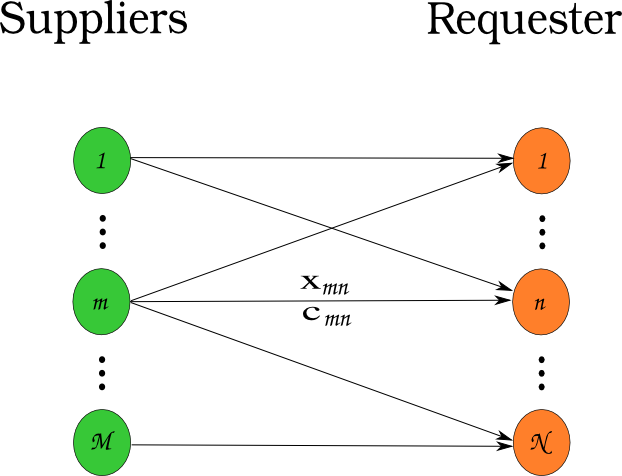
\includegraphics[height=5cm]{./images/xportation.eps}
      \caption{A Pictoral View of the Transportation Problem.}
    \end{figure}

\end{frame}

\begin{frame}[ctb!]
  \frametitle{Linear Programming}

  General form:

  \begin{subequations}
    \begin{align}
      \min \: & \sum c x \\
      \text{s.t.} \: & A x \leq b \\
                     & x   \geq 0
    \end{align}
  \end{subequations}
  
\end{frame}

%% \begin{frame}[ctb!]
%%   \frametitle{The Simplex Method}

%%     \begin{figure}
%%       \includegraphics<1>[height=5cm]{./images/geometric.eps}
%%       \includegraphics<2>[height=5cm]{./images/rotated.eps}
%%       \caption{A Pictoral View of the Simplex Method.}
%%     \end{figure}
%% \end{frame}

\begin{frame}[ctb!]
  \frametitle{Integer Programming}

  General form:

  \begin{subequations}
    \begin{align}
      \min \: & \sum c x \\
      \text{s.t.} \: & A x \leq b \\
                     & x   \geq 0 \\
                     & x_i \in \mathbb{Z} \forall i \in I 
    \end{align}
  \end{subequations}
    
\end{frame}

%% \begin{frame}[ctb!]
%%   \frametitle{Branch and Bound}
  
%% \end{frame}
